\chapter{INTERFACE IMPLEMENTATION}
\label{chap:GUI_impl.tex}
\section{INTERFACE}
The necessity to enhance manual debug methodology has been established in Section~\ref{sec:enhancement.tex.nemv} and certain requirements of such an interface is established in Section~\ref{sec:enhancement.tex.emv}. This chapter concentrates on design and implementation of the debug interface.

The debug interface is aimed at being intuitive and user friendly. It should aid data navigation so as to reduce manual efforts. If user requires to refer to actual processor execution log or assembly code, it should be readily availalbe through the interface. The interface should also provide graphical representation of processor execution log, to aid traversal and filtering of processor activity. The interface should aid traversing through processor execution easy.  Critical events made by processor should be extracted, categorized and made availabe to user.

In addition to interface requirements listed in Section~\ref{sec:enhancement.tex.emv}, the following set of features would also aid in debug:

\begin{itemize}
\item[-] Visualizing thread-wise execution flow
\item[-] Ability to highlight instances of critical activities such as Memory write/read, I/O write/read, Branching etc
\item[-] Interrupt and exception happening during execution
\item[-] Assembly code traversal and its linkage with execution flow
\item[-] Register current state value traversal and its linkage with execution flow
\item[-] Comparison of register values between arbitrary instances of execution
\item[-] Simulation cycle of execution event
\end{itemize}

Every stimulus is a unique assembly test and hence the debug interface should be as generic as possible. It should be able to accomodate any relevant assembly test, accompanied with execution logs.

%Once the simulation is completed and failure is reported the debug phase starts. This is where the role of GUI comes. From the vast information provided by the logs and test files, interfaces have to capture and represent relevant information to the user. The following section details the implementation and features of the proposed GUI. 

\subsection {CHOOSING GUI}
There are multitude of languages providing GUI capability, the project doesnot need a very sophisticated GUI implementation. Moreover the interface should aid remote debug and if possible thee should not be any requirement for any user to install a tool-kit or library for the debug interface to be used. Hence the decision to use web-browser as the debug interface was a default choice. A web browser could also execute {\it javascripts} and that makes it customisable. The design is also scalable and aids introduction of new features for debug with ease.

Each stimulus will have its own set of assembly test files and execution log files. The interfaces implementation starts by consuming these files. Two programming languages are used for implementation:
\begin{description}
\item[Python Script] for data extraction and correlating related information.
\item[JavaScript] for designing the interface features and user interaction.
\end{description}

\addtocontents{toc}{\protect\setcounter{tocdepth}{2}}
%\figurename{} 
\begin{figure}[h]
\centering
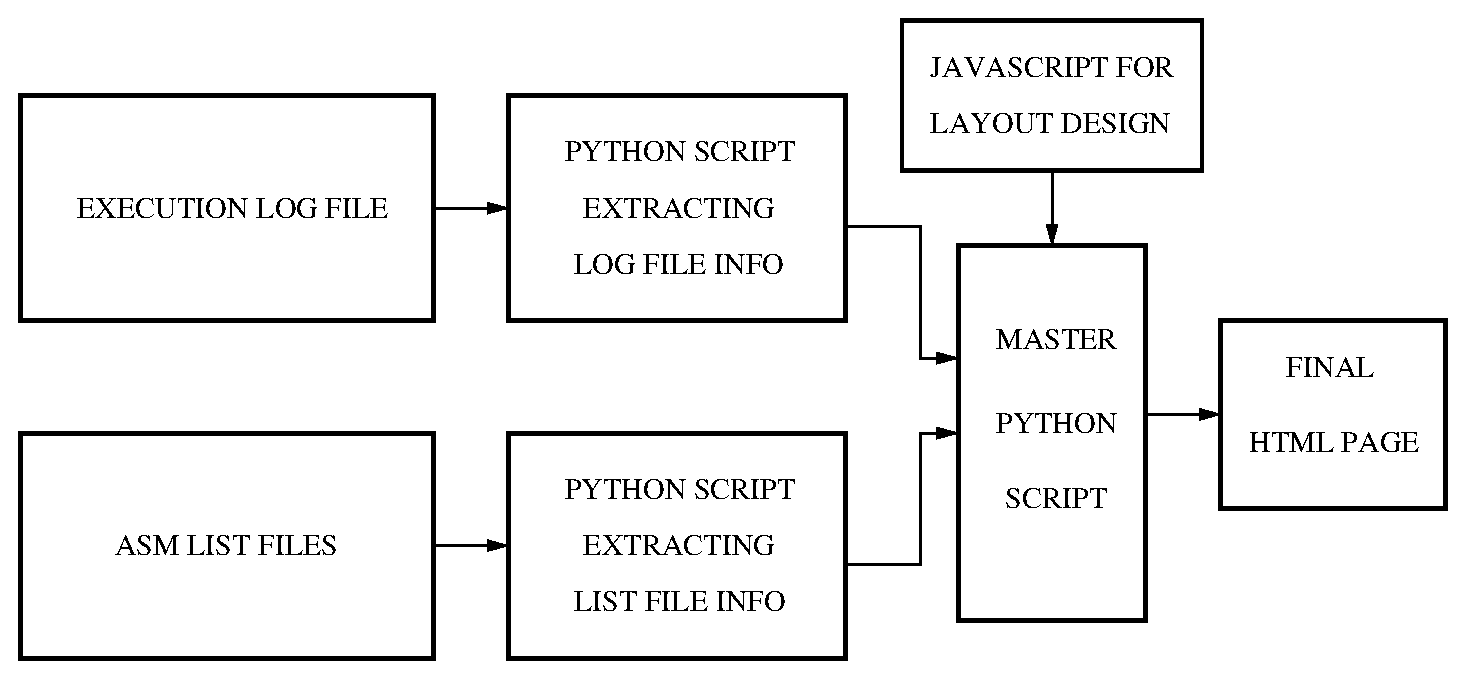
\includegraphics[width=5.5in]{./figures/gui_impl.eps}
\caption{GUI Implementation} 
\label{fig:gui_impl.eps}
\end{figure}

Figure~\ref{fig:gui_impl.eps} depicts information extraction and use of different scripts to achieve the same. Major implementation steps
\begin{itemize}
\item[-] Extraction of information from assembly list file and processor execution log by python script.
\item[-] Correlation of information from previous step.
\item[-] Coding generic JavaScript code for user interactions.
\item[-] Top level python program to manipulate available information and to convert it to JavaScript information. 
\item[-] The top level python program will combine the data extracted and javascriot code to generate a single HTML page. 
\end{itemize}

The whole infrastructure is packaged neatly. Given execution log file and assembly list file, the top level python script generates the HTML interface web page. Different stages involved in this conversions are described in the following sections. 

\subsection {INTERFACE}
GUI is targetted to run on any browser, hence layout design is done using {\it HTML}\nomenclature{HTML}{Hyper Text Markup Language}. However for providing interactive features to the user, a much more powerful language is need along with HTML and default choice is JavaScript.

\emph {\bf JavaScript (JS)} is an interpreted computer programming language. It is  implemented as part of web browsers so that client-side scripts could react to user inputs, customize the browser, communicate asynchronously, and to filter contents being displayed. It is a multi-paradigm language, supporting object-oriented, imperative, and functional programming styles.  
In addition a style sheet language called CSS\nomenclature{CSS}{Cascading Style Sheets} is used for describing the presentation semantics (the look and formatting) of the interface page written in HTML.

%\figurename{} 
%\figurename{} 
\begin{figure}[h]
\centering
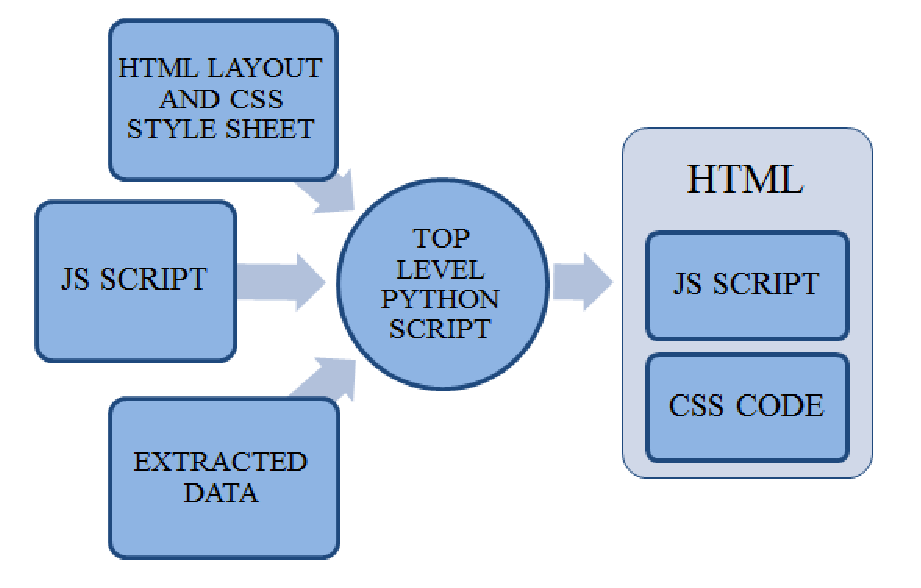
\includegraphics[width=3.5in]{./figures/html.ps}
\caption{Web Page Generation}
\label{fig:impl:wpg}
\end{figure}

Resultant HTML page embeds JavaScript routines and style sheets. This is done by the top level python script. Figure~\ref{fig:impl:wgp} shows a representation of information flow.


\subsection{JS DATASTRUCTURE}
All dynamic features of the interface are handled by JS\nomenclature{JS}{JavaScript} script routines. Data input to the JS is the extracted information from execution log files and list files. The top level python script converts the extracted objects into JS data array ``$dataArray[]$'' ; where each array element coresponds to an active thread. Active threads refer to active core or processor in a multiprocessor system.  

\IncMargin{1em}
\begin{algorithm}[h]
\DontPrintSemicolon
\SetKwInOut{Input}{Input}\SetKwInOut{Output}{Output} \SetKwFunction{KwFn}{CreateDataArray}
\KwFn {}
\BlankLine
\Begin{
\For {i in activeThreads}{\;
		\For {$log$ in logObj}{\;
		\If{log.Id == i}{
		Append $log \rightarrow	DataArray[i]$\;
		}
}
}
}
\caption{Creating JavaScript Object}
\end{algorithm}\DecMargin{1em}



Once the extracted information is converted to JS compatiable data, the interface features can utilize this. The layout for various GUI features called windows, are designed using HTML and CSS code. All dynamic interactive featurers are handled by embedded JS script in HTML web page. Later sections introduces different windows availabe in the web page.

\section {EXTRACTION OF INFORMATION}
The first step in creating a generic debug interface is to extract relevant information and convert it to a format that could be loaded by the debug interface.

\subsection {STIMULUS}
Stimulus is written in X-86 assembly language. The engineer is expected to debug this stimulus. Each cycle in processor execution log corresponds to a particular assembly code. An assembler is used to assemble to object code, in that process each instruction is also mapped to a particular address. Figure~\ref{impl.tex:assembler} shows this process which also produces a list file which hold an macro expanded, loop unrolled, assembled code with corresponding address details. The configuration file defines certain random operands, segmentation, gdt, ldt, page tables to aid in assembling process. The include files contribute common routines used across different assembly stimuluses.

%However, the written by the verification engineer is the unscheduled code without any memory address details. For cycle comparison with execution log, the asm test file is complied first.

\begin{figure}[h]
\centering
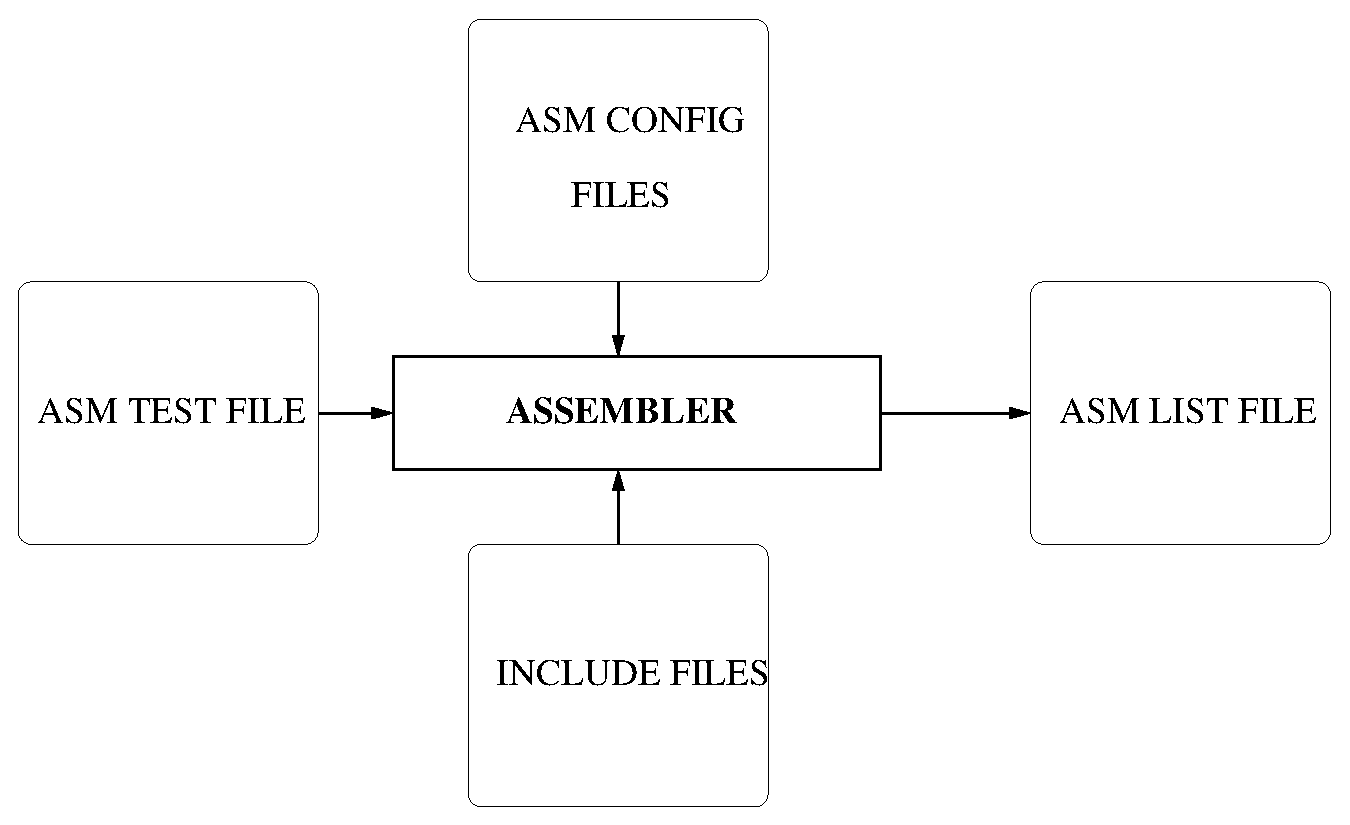
\includegraphics[width=3.5in]{./figures/asm.ps}
\caption{Assembler}
\label{impl.tex:assembler}
\end{figure}


\begin{figure}[h]
\centering
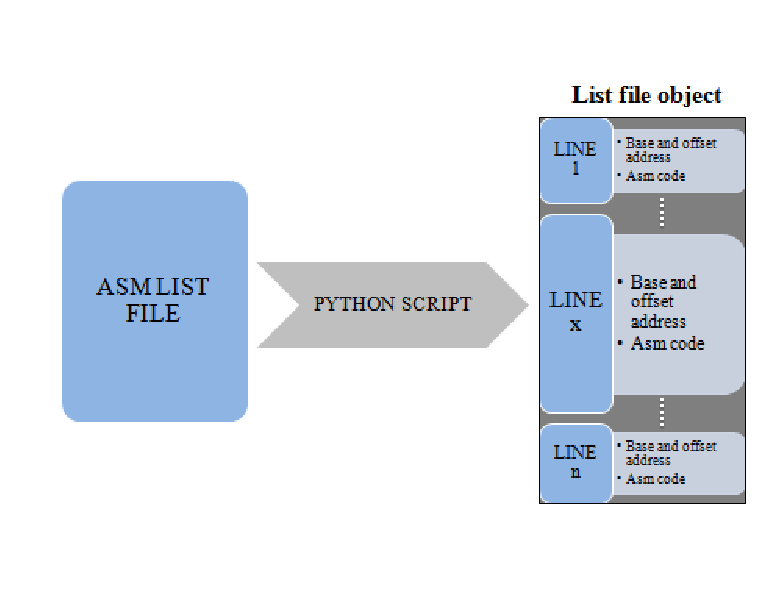
\includegraphics[width=4.5in]{./figures/list.ps}
\caption{Asm List File Extraction}
\label{impl.tex:listextr}
\end{figure}

List file holds a wealth of details including instructions, opcodes, operand, linear address, module/register configuration details etc. A {\it python} script is used to extract relevant information corresponding to each instruction line in the list file. In this project, the following information is extracted for each instruction from the  list file:
\begin{itemize}
	\item[-] Base and offset address value
	\item[-] Instruction line number
	\item[-] The assembly code
\end{itemize}

The {\it python} script internally contains a data structure of list objects, which helps in adding features to the script with ease (Figure~\ref{impl.tex:listextr}). 

\subsection {EXECUTION LOG}
Execution log file contains instruction by instruction execution details from simulation. It also includes register states, thread details, flag values and other details which help in tracing out the cause of failure. As explained in previous chapters, debugging require detail traversal through this log file. 

Details in the log file with reference to each cycle is required to be extracted. {\it Python} script is used to extract these informations as well and a comprehensive data structure is created. The data structure objects contain properties corresponding to major operations and register values. Thread details are handled as seperate data structures as it aids processing thread-wise informations. Following properties are extracted from execution log file for every execution event

%Figure x shows how the script will read the input execution log file and generate log file objects.

\begin{itemize}
 \item[-]  Thread number
 \item[-]  Mode of operation
 \item[-]  Cycle number
 \item[-]  Linear address
 \item[-]  Memory write, Memory read, I/O write/read, Code read
 \item[-]  Branch target (linear address)
 \item[-]  New values of registers, if modified
\end{itemize}


\subsection {INFORMATION CORRELATION}

Once both the input files are processed, next step is to correlate assembly with execution log. A {\it python} script can accompish this by correlating respective data structures based on linear addresses. As x86 architecture follows segmented memory model along with paging, address translation is required for generating the linear/physical address\cite{SS:AMD64-V2}. Linear address is calculated as
\\
\centerline{Linear address = Base address + Offset value}
\\


%\vspace{1.5cm}

\IncMargin{1em}
\begin{algorithm}[h]
\DontPrintSemicolon
\SetKwInOut{Input}{Input}\SetKwInOut{Output}{Output} \SetKwFunction{KwFn}{CreateDataArray}

\Input{list file objects$\rightarrow listObj[]$, log file object$\rightarrow logObj[]$}
\BlankLine
Start: \;
\For {each object $list$ in listObj}{\;
		list.address = list.Base + list.Offset\;
	}
\For {each object $log$ in logObj}{\;
	set count = 0\;
	\For {each object $list$ in listObj}{\;
	 \If{$log.address == list.address$}{
		Append each $list$.property $\rightarrow$ $log$.property\; \tcp{$log$ properties are lineNo, opcode and address}\label{cmt}
		count = 1;
		break loop\;
	}
	}
	\If{count == 0}{
	assert: $"no address match"$
	}
}
End \;
\caption{Combining List and Log File Information}
\label{impl:algo:cllf}
\end{algorithm}\DecMargin{1em}

%\vspace{1.5cm}

For each object of execution log, the corresponding list file object could be found based on linear address value. Once found, both are cross-linked to aid further processing. The alogorithm employed in this search is depicted in Algorithm~\ref{impl:algo:cllf}. Data extraction is complete with this linkage and the result is execution log objects linked to corresponding assembly objects.

\section {GUI FEATURES}

\subsection {EXECUTION FLOW GRAPH}
Main feature of the web page is the graph showing the execution flow of the code. Here asm list file line numbers are plotted against the cycle during which it is executed. All the active threads have different graphs which are tabbed. Hovering the mouse over any point on the graph will display x and y axis values. 
 
This zoom enabled data graphs also provides onclick selection of specific operations e.g: Branching, Memory Write, Memory Read, Code Read etc, which will display the instances of selected operation. Each operation is distinguished by its color.   

\subsubsection {Implementation}

For the developement of execution graph we are using Dygraph JavaScript Visualization Library []. This will provide inbuild functions that enable zooming, x-y axis value display and point onClick call backs. onClick CallBack() function is called when ever a point on Dygraph is clicke and this function actives many other window.

For building the graph, input to the Dygraph is independent axis values followed by depended axis values. For each thread, a different graph is generated. The x-axis is cycle number and y-axis is the list file line number. Algorithm x explains hw the graph is build.

\IncMargin{1em}
\begin{algorithm}[h]
\DontPrintSemicolon
\SetKwInOut{Input}{Input}\SetKwInOut{Output}{Output} \SetKwFunction{KwFn}{CreateGraph}
\KwFn{}
\BlankLine
\Begin{
\For {each i in activeThread}{\;
\For {each element in dataArray[i]}{\;
	Dygraph[i] $\leftarrow [element.cycleNo , element.lineNo]$\;
	}
}
}
\caption{Creating Execution Graph}
\end{algorithm}\DecMargin{1em}

\section {REGISTER WATCH WINDOW}

Register window capture and display updated register values at a specific instance. Each thread holds its own copy of registers/flags. A selection of point on the execution flow graph will update the register window with values at that instant in the selected thread. Values of following registers and flags are provided to the user:
\begin{itemize}
	\item[-] 64 bit general purpose registers (RAX, RBX, RCX etc)
	\item[-] RFLAG (64 bit)
	\item[-] Instruction Pointer (RIP)
	\item[-] Stack Pointer (RSP)
\end{itemize}

Another feature provided by register window is comparison between register values at two different instances that is between a reference point set by Set Marker button and current selection. 

\subsubsection{Implementation}

This window is activated by the point onClick CallBack function evoked when a point is clicked on Dygraph. The function will update the register window rows set by the HTML code eg. regRow[RFLAG], regRow[RBX] etc. Also there will be a comparison with the reference point set. 

\IncMargin{1em}
\begin{algorithm}[h]
\DontPrintSemicolon
\SetKwInOut{Input}{Input}\SetKwInOut{Output}{Output} \SetKwFunction{KwFn}{pointonClickCallBack}
\KwFn{element}
\BlankLine
\Begin{
\For {each reg in RegisterSet}{
regRow$[reg]$ $\leftarrow$ element.$[reg]$ \;
	\If{(element.$[reg]$ != referenceRow.$[reg]$)}{\;
		$Highlight  regRow $ \;
	}
}
}
\caption{Creating Register Window}
\end{algorithm}\DecMargin{1em}

\subsection {INSTRUCTION WINDOW}

Instruction window give the asm file lines. A selection in execution graph will be reflected in this window by highlighting the asm file instruction corresponding to the selected point. Also the context of the selected line that is its preceding and succeeding instructions are also available in this window.
\subsubsection{Implementation}

This window is also activated by the onClick CallBack function evoked when a point is clicked on Dygraph. The function will update the instruction window set by the HTML code.

\IncMargin{1em}
\begin{algorithm}[h]
\DontPrintSemicolon
\SetKwInOut{Input}{Input}\SetKwInOut{Output}{Output} \SetKwFunction{KwFn}{onClickCallBack}
\KwFn{element}{;\
\BlankLine
\Begin{
\For {each item from elemnt-50 to element+50}{\;
	Add $item.opcode \rightarrow$ InstructionWindow\;
	}

Add $item.logInfo \rightarrow$ ExecutionLogWindow\;
}
}
\caption{Creating Instruction and Execution Log Window}
\end{algorithm}\DecMargin{1em}

\subsection {EXECUTION LOG WINDOW}

In addition to the instruction and register information, all the processor execution log information regarding the selected
instruction is also provided through execution log window.  This collected information is stored as a log file object propert "{\emph logInfo}". 

Implementation of Execution log window is given in algorithm x along with instruction window.

\subsection{SET AND CLEAR MARKER}
These two options allow setting or removing a reference point with which current register values are compared against.

\subsubsection{Implementation}

Set and Clear buttons are set using HTML form options. These elements have onClick call backs. On clicking Setbutton call back will set add values to reference register section and on click clear will remove the values in reference section.



